\section{Hardware Choice} \label{Hardwarechoice}
Hardware components are chosen from the Requirements (see \secref{Requirements}) to build a prototype. 
Some of the hardware components are given with the vehicle (the servo used for steering and the Hall sensors used for velocity measurement) and therefore, aren't described in this section. 
Besides the requirements, the availability of the components and their compatibility with the system have to be considered.

%%%%%%%%%%%%%%%%%%%%%%%%%%%%%%%%%%%%%%%%%%%%%%%%%%%%%

\subsection{Microcontroller}
The microcontroller is the brain of the system. The purpose of the microcontroller is to connect all the other hardware components. It also contains the software code necessary to control the rest of the system by sending and receiving electrical signals as needed.

The requirements for the microcontroller are:
\begin{itemize}
% \item Having a CPU, that has a frequency greater than \si{XX\ MHz}. \todo{Number}
\item Having I/O connections, both digital and analogue.
\item Having output connections, that can transmit PWM signals.
\item Having 5 free timers,\todo{Where do we have this number from (in the report)?} to run and control the different parts of the system in parallel.
\item Being powered by an external power source.\todo{?}
\end{itemize}

\subsubsection{Arduino Mega 2560}
The Arduino Mega 2560 is a microcontroller board, which comes with an 8-bit ATmega2560 integrated circuit and extends its I/O ports, see \figref{ArduinoMega} \cite{MegaInfo}. 

\begin{figure}[H]
	\centering
	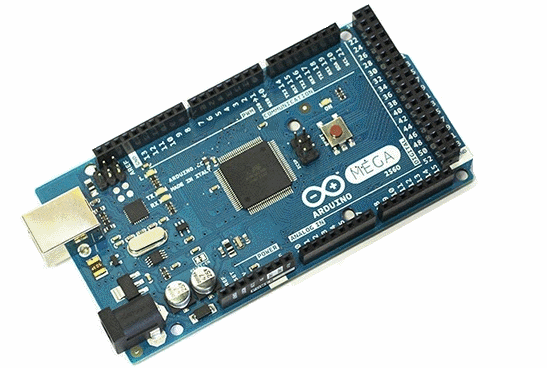
\includegraphics[width=0.5\textwidth]{figures/ArduinoMega.png}
		\caption{An Arduino Mega 2560 board [source: Arduino site]} 
	\label{ArduinoMega}
\end{figure}
%
It has \si{54} digital ports with a 5 volts logic. From these, \si{15} can be used to generate PWM signals. The CPU runs at \si{16 MHz} and the chip has \si{6} integrated timers, one of which is used by the Arduino itself. There are also 4 UARTs, used in serial communication, as well as a setup for SPI communication and an \si{I^2C} bus. The Arduino can be powered though a USB cable or with an external power source.

The Arduino Mega board is the one that is used in this project, since it ships with all the connections needed to use the already chosen hardware and has many different types of connections to set up the other hardware components. The Arduino is programmable through a serial connection, with the help of avrdude\cite{Avrdude} or simply through the Arduino IDE\cite{ArduinoIDE} which can compile C, C++ and Arduino (syntax very close to C and C++) files.\\
%
By chosing this Arduino microcontroller board as the central hardware component, the rest of them need to be compatible with it.

%%%%%%%%%%%%%%%%%%%-STORAGE-%%%%%%%%%%%%%%%%%%%%%%

\subsection{Storage}
The storage is used for saving the edge map and the route planned for the vehicle. All this data have to be saved from one usage to the other.

The requirements for the storage are:
\begin{itemize}
\item Having to be controlled by the microcontroller.
\item Offering the possiblity to retrieve the stored data after a power cut to the storage.
\item Having a storage of \si{XX\ MB}. \todo{Number}
\item Having a transfer speed greater than \si{XX\ B/s}. \todo{ref}
\end{itemize}

\subsubsection{SD Card} \label{SDcard}
Secure Digital (SD) card is a type of non-volatile flash memory cards. This means that the data will not be lost during a power cut off.\\
%
It comes in various storage sizes, from 1 GB to 2 TB, depending on which type of SD card it is. There is 3 types of SD card, the standard capacity (SDSC), the high capacity (SDHC) and the extended capacity (SDXC). The  difference between the different type, is the file system use on the card and the maximum capacity. With the requirement of a storage size on XX bytes, the SDSC is big enough with a capacity of 2 GB.\\
%
The lowest transfer speed for an SDSC card is \si{2 MB/s}. With the requirement of a transfer speed greater than \si{XX\ bit/s}, the SDSC card is fast enough. 

To use the SDSC card and connect it to the microcontroller, 7 connection pins are required, see \figref{SDcardpinout}. The setup of the SD card is different, depended on which mode is used.

\begin{minipage}{\linewidth}
      \centering
      \begin{minipage}{0.65\linewidth}
			\begin{table} [H]
				\begin{tabular}{|l|l|l|l|}
								
\hline
\textbf{Pin} & \textbf{SPI}  		& \textbf{One bit} 	& 	\textbf{Four bit}  \\
\hline
1			 &	Unused		 		&	Unused			    &	Data 2			   \\
\hline
2			 &	Card Select	 		&	Card Detection		&	Data 3			   \\
\hline
3			 &	Data In		 		&	\begin{tabular}{@{}l@{}} Command \&  \\Response \end{tabular}  &	\begin{tabular}{@{}l@{}} Command \&  \\Response \end{tabular} \\
\hline
4			 &	Power 				&	Power			    &	Power			   \\
\hline
5			 &	Serial clock 		&	Serial clock		&	Serial clock	   \\
\hline
6			 &	Ground		 		&	Ground			    &	Ground			   \\
\hline
7			 &	Data Out	 		&	Data 0			    &	Data 0			   \\
\hline
8			 &	Unused		 		&	Unused			    &	Data 1			   \\
\hline		
				\end{tabular}
				\caption{SD card pinout configuration}							
			\end{table}			
      \end{minipage}
      \hspace{0.03\linewidth}
      \begin{minipage}{0.30\linewidth}
          \begin{figure}[H]
              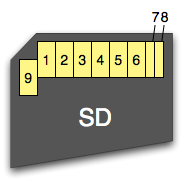
\includegraphics[width=0.95\textwidth]{figures/sdcardpinout}
              \caption{Illustration of a micro size SD card.} % http://elasticsheep.com/2010/01/reading-an-sd-card-with-an-atmega168/
              \label{SDcardpinout}
          \end{figure}
      \end{minipage}
      
  \end{minipage}

The power needed for a SD card is 3.3 volts. There are three possible setups for the SD card: SPI, One-Bit and Four-Bit.
With the SPI setup, the communication between the SD card and the microcontroller is made on two lines. The SPI mode is the most used one for embedded systems.\todo{source !}
With the One-Bit setup, the commands between the SD card and microcontroller are sent on one line and the data is sent though another one.
With the Four-Bit setup, three more data connections are used.\\
%
In this project, the SPI setup is used, as it is the most used method and the extra transfer speed from the Four-Bit setup is not needed. Furthermore, the Arduino has 4 pins that can be set up to SPI communication.\\

The choice for this project is made towards an SDSC card, with a SPI setup, as the capacity and transfer speed meet the requirements. The data will be saved, if the power is cut off. The last requirement, the connections to the microcontroller, is possible since the Arduino Mega 2560 controller contains digital I/O pins, that can be used for the SPI setup of the SD card.

%https://www.sdcard.org/developers/overview/capacity/index.html
%https://www.sdcard.org/developers/overview/speed_class/

%%%%%%%%%%%%%%%-Motor Driver-%%%%%%%%%%%%%%%%%%%%

\subsection{Motor Driver}
The motor driver is the connection between the microcontroller, the power supply and the motor. It is used, to isolate the hardware components functioning in low power, i.e. the microcontroller, from the high power parts, i.e. the motor.

The requirements for the motor driver are:
\begin{itemize}
\item Having to be controlled by the microcontroller.
\item Offering the possibility to power it through an external power source.
\item Being able to handle the battery pack's voltage.
\item Allowing to power the motor in both direction.
\end{itemize}

\subsubsection{Pololu Dual VNH5019}
The Pololu dual VHN5019 motor driver shield (see \figref{MotorDrive}) is specially designed for Arduino boards. It can be placed directly on top of the the Arduino board as a shield, with the pins connecting to the right ports on the Arduino. 

\begin{figure}[H]
	\centering
	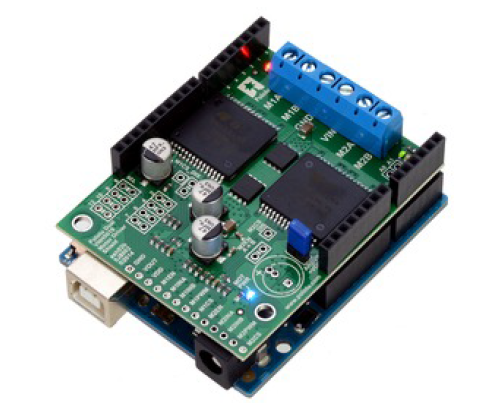
\includegraphics[width=0.50\textwidth]{figures/Motordriver.png}
		\caption{The motor shield on top of an Arduino Uno.} 
	\label{MotorDrive}
\end{figure}

It is possible to power the Arduino from an external power source through the motor shield, which also delivers the power to the motor. It is also possible to have the motor shield and the Arduino powered separately. This is determined by a jumper setting on the shield, see \figref{MotorDriveIO}. The motor shield need a power voltage between 7 volts and 12 volts.

\begin{figure}[H]
	\centering
	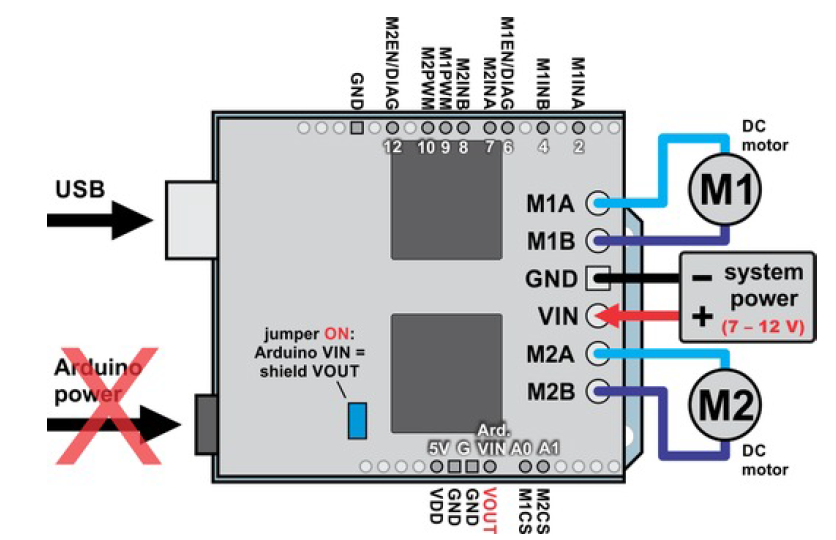
\includegraphics[width=0.60\textwidth]{figures/MotordriverIO.png}
		\caption{Setup for the mort shield.}
	\label{MotorDriveIO}
\end{figure}

There are two H-bridges \todo{secref{sec:HBridge}}on the board, to control up to two motors. Since only one motor is used in this project, the two H-bridges will be used in parallel to power the motor. This should result in a smaller current through the two H-bridges' transistors and therefore ensure a better protection of the system.

\begin{figure}[H]
	\centering
	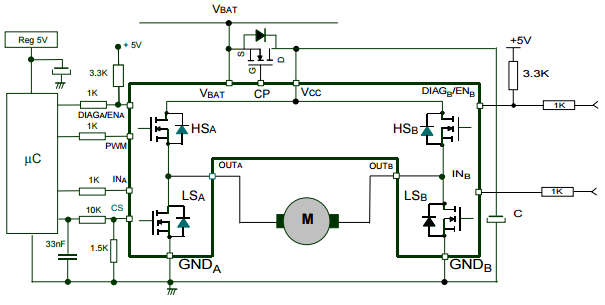
\includegraphics[width=0.85\textwidth]{figures/Hbridges.png}
		\caption{Illustration of the H-bridge, that the motor shield have two of.}
	\label{Hbridges}
\end{figure}
%
Each one of the H-bridges is controlled by a PWM signal from the Arduino. However, as the two H-bridges are combined into one, only one is controlled by a PWM signal. This is done by putting both H-bridges into cruise mode, one to high and the other to ground. Then the PWM signal sent to the H-bridge, that is set to high, will regulate the voltage sent through the motor. If needed to reverse the voltage across the motor, the settings for the two H-bridges shall be swapped around.

The Pololu dual VHN5019 motor driver shield is used in this project, as it is made for the Arduino and therefore easy to implement. Moreover, it can power the Arduino through an external power source and get a power output high enough for the motor and in each direction.

%Source: The datasheet

%%%%%%%%%%%%%%%%%%%%%%%%%%%%%%%%%%%%%%%%%%%%%%%%%%%%%

\subsection{Wireless communication system}
The data from the GoT system is sent to the microcontroller with this comunication system. The transmitter will be located on the computer used for the GoT system and the receiver on the vehicle. As the prototype will be tested in the control lab, the distance that the wireless communication have to send is less than 10 meters.

The requirements for the wireless communication components are:
\begin{itemize}
\item Having to be controlled by the microcontroller.
\item Having a range greater than 10 meters. 
\item Offering the possibility to be powered by an external power supply (through the Arduino power lines).
\item Transfering at a higher rate than \si{120\ B/s}. \todo{ref}
\item Offering the possibility to control it and couple it with the GoT code.
\end{itemize}

\subsubsection{Xbee}\label{Xbee}
Xbees are small radio modules, that are easy to set up. An overview of the Xbee and its pin layout can be seen on \figref{XbeeLook} and \figref{Xbeepinout}.


\begin{minipage}{\linewidth}
	\centering
	\begin{minipage}{0.45\linewidth}      
		\begin{figure}[H]
			\centering
			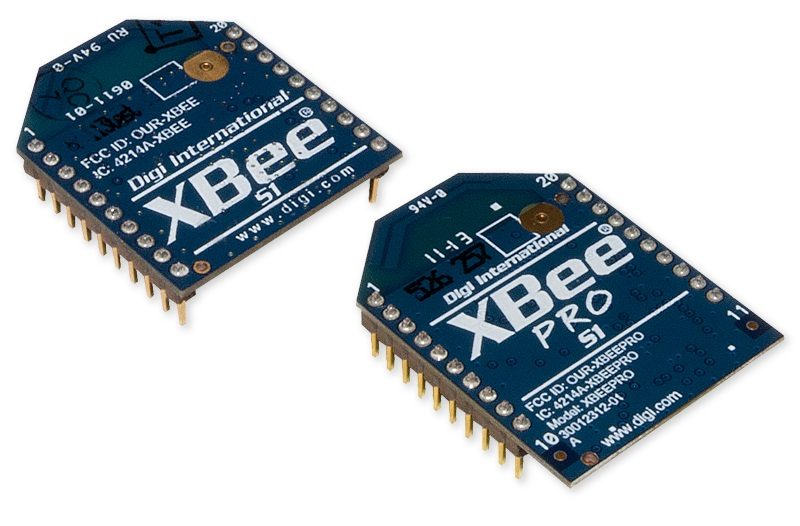
\includegraphics[width=0.95\textwidth]{figures/Xbee.jpg}
			\caption{Two Xbee radio modules} 
			\label{XbeeLook}
		\end{figure}
	\end{minipage}
	\hspace{0.03\linewidth}
	\begin{minipage}{0.45\linewidth}
		\begin{figure}[H]
			\centering
			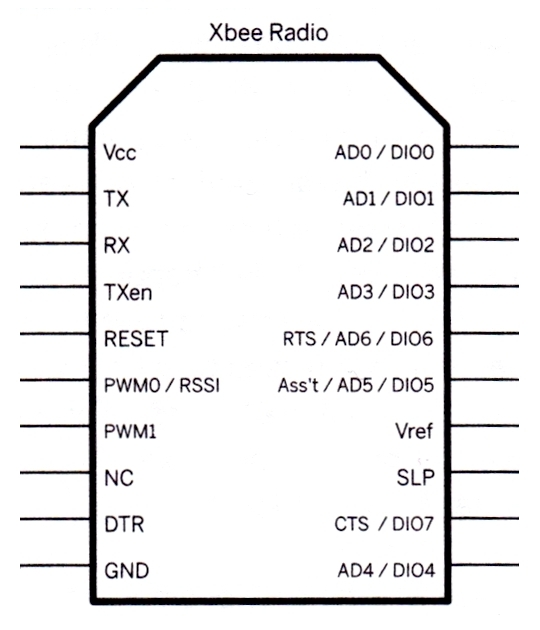
\includegraphics[width=0.95\textwidth]{figures/XbeeIO.jpg}
			\caption{Pinout of an Xbee radio module} 
			\label{Xbeepinout}
		\end{figure}
	\end{minipage}
\end{minipage}

\todo{Snak med vinkel om at få teksten align}

The Xbee modules communicate through an UART connection (with TX and RX pins). Since the Arduino has three UART connections plus the one used to program the Arduino, the Xbee can be connected. The software code for the GoT system is implemented in C\# (see in \secref{GoTDescription}) and the computer running has serial ports that can ensure the connection between the software and the Xbee. Therefore, this solution can be used for a wireless connection between the GoT system and the Arduino.

To run the Xbee modules, a \si{3,3\ V} power line, a ground line, and a \si{3,3\ V} logic UART are needed. The rest of the pins are not needed in this project. The modules have a transfer speed of up to \si{115,2 kbit/s} and can reach up to \si{100 m} indoor and \si{300 m} outdoor. It transmits at a \si{2,4 GHz} frequency with \si{1 mV} (\si{0 dBm}) and can receive downto \si{-96 dBm}. The Xbee is already ready for communication, with the lower levels of communication, the physical and data link layers, being already implemented. With only two devices, a lightweight combination of transport and presentation layer can be added to the protocol directly on top of the data link layer, to add more error handling and to set up how the data shall be sent.

%http://www.digi.com/products/xbee-rf-solutions/modules/xbee-digimesh-2-4#specifications

%%%%%%%%%%%%%%%%%%%%%%%%%%%%%%%%%%%%%%%%%%%%%%%%%%%%%

\subsection{Angular sensor}
The angular sensor is used in the feedback for the control system.

The requirements for the angular sensor are:
\begin{itemize}
\item To be controlled by the microcontroller.
\item Having a sampling frequency greater than XX. \todo{Number}
\item Having a latency smaller than XX. \todo{Number}
\item Offering the possibility to power it by an external power supply (through the Arduino power lines).
\end{itemize}

\subsubsection{HMC5883L}
Sparkfun's "9 degrees of freedom" board comprises a magnetometer integrated circuit, the HMC5883L\cite{HMC5883L}. A magnetometer will be used as the angular sensor, since it can be set up as a compass and give out a angle compared to north. As the direction to north is always the same, the system does not need a new calibration of the angular sensor, if used in a new area. However, it has to be calibrated on the vehicle when used for the first time.

\begin{figure}[H]
	\centering
	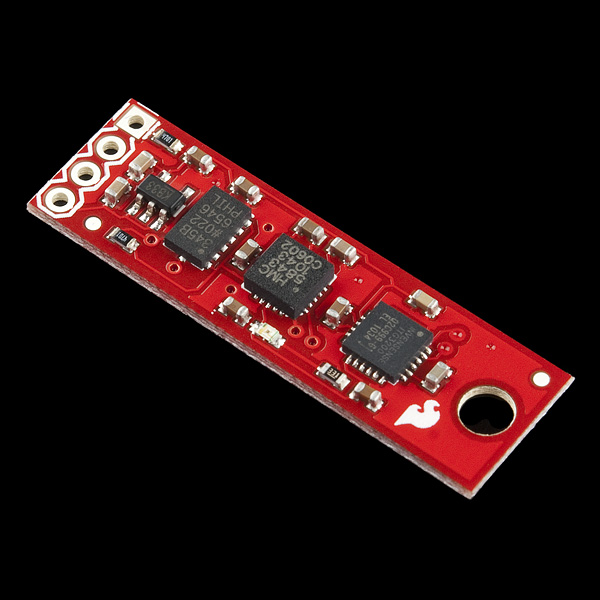
\includegraphics[width=0.50\textwidth]{figures/NineDegree.jpg}
		\caption{Sparksfun's "9 degrees of freedom" sensor stick} 
	\label{NineDegree}
\end{figure}

The "9 degrees of freedom" sensor stick, see \figref{NineDegree}, will be used in the project. Beside the magnetometer, there are also a accelerometer and a gyroscope on the board, but these will not be used. The "9 degrees of freedom" sensor stick is designed to be used with a microcontroller and comes with software example for the Arduino platform. It needs an  \si{I^2C} bus to communicate with the Arduino, which has that kind of interface.

%%%%%%%%%%%%%%%%%%%%%%%%%%%%%%%%%%%%%%%%%%%%%%%%%%%%%

\subsection{Power monitor}
The power monitor is used to give a feedback to the system about the level of power in the battery pack.

The requirements for the angular sensor are:
\begin{itemize}
\item Being monitored by the microcontroller.
\item Measuring the battery pack voltage output downto \si{5,7\ V}.\todo{ref}
\end{itemize}

\subsubsection{Voltage divider}
A voltage divider is an electronic circuit, that divides the input voltage with a constant depending on the values of the resistors used in the circuit, see \figref{VoltDivFig}.

\begin{figure}[h!]
\centering
\begin{circuitikz}
\draw (0,0)
to[V,v=$V_{in}$] (0,2)
to[short] (2,2)
to[R=$R_1$] (2,0)
to[R=$R_2$] (2,-2)
to[short] (0,-2)
to[short] (0,0);
\draw (2,-2) 
to[short] node[ground] {} (2,-3);
\draw (2,0)
to[short] (3,0)
to[short,l=$V_{out}$] (4,0);
\end{circuitikz}
\caption{Standard voltage divider} 
\label{VoltDivFig}
\end{figure}

The output of the voltage divider can be find with \eqref{VoltageDivider}. 

\begin{flalign}
\eq{V_{out}}{\frac{R_2}{R_1 + R_2} \cdot V_{in}}\unit{V} 
\label{VoltageDivider}
\end{flalign}
\hspace{6mm} Where:\\
\begin{tabular}{p{1cm}lll}
& \si{V_{in}} & is the battery pack voltage &\unitWh{V} \\
& \si{R_1, R_2} & are two calculated resistors &\unitWh{\Omega}\\
& \si{V_{out}} & is the measured output voltage &\unitWh{V}
\end{tabular}

The input voltage is set to be the battery pack and the output is measured though an analogue pin on the Arduino. The analogue pin on the Arduino can measure from \si{0\ V} to \si{5\ V} with a resolution of \si{10\ bits}. This gives 1023 steps from 0 to 5 volts and each step is \si{4,9\ mV}. The size of each step and the range for the measuring is multiplied with the inverse constant, that comes from the two resistor, so it is possible to make the range go over \si{5\ V}. 

A voltage divider is used in this project, as it can be scaled to the interval that it has to measure. The voltage divider will be connected to an analogue pin on the Arduino, which will make the measurement from the output of the voltage divider.\\

From the requirements for the system to the hardware parts, these components have been chosen. After having chosen the different hardware components for the prototype, the different components have to be implemented in the system.
%%%%%%%%%%%%%%%%%%%%%%%%%%%%%%%%%%%%%%%%%%%%%%%%%%%%%


%Pins on the arduino
%SD card (4 I/O)
%Xbee (1 TX and 1 RX)
%Hall (2 I/O)
%Angular (1 SDL and 1 SDA)
%Servo (1 PWM)
%Motor (1 PWM)
